\documentclass[tikz,border=8pt]{standalone}
\usepackage{amsmath,amssymb}
\usepackage{tikz}
\usetikzlibrary{arrows.meta,calc,decorations.pathreplacing,patterns,shapes.geometric,positioning,shadings}

\begin{document}
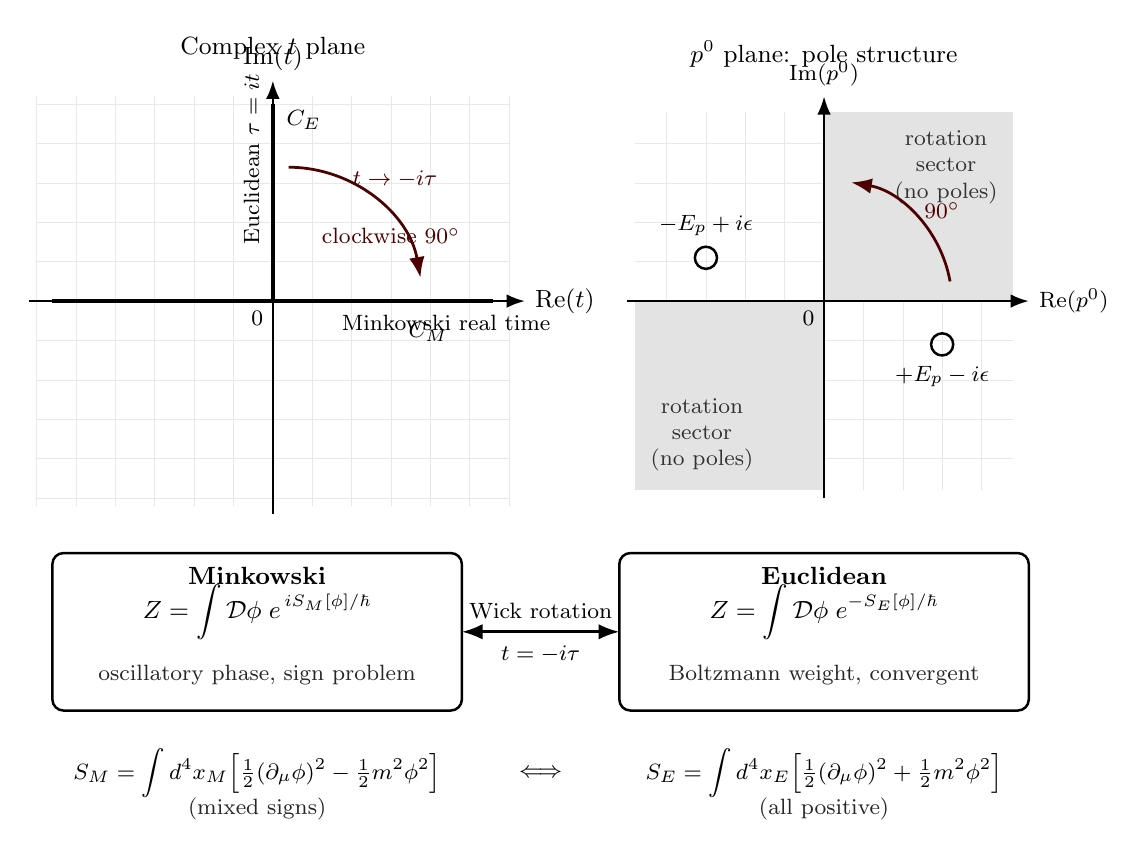
\begin{tikzpicture}[>=Latex, font=\small]

% =====================================================================
% TOP PART: complex t plane with Wick rotation
% =====================================================================

\begin{scope}[shift={(-3.4,3.6)}]
  % Light grid background
  \draw[step=0.5cm, gray!18, very thin] (-3.0,-2.6) grid (3.0,2.6);

  % Axes
  \draw[->, thick, black] (-3.1,0) -- (3.2,0)
     node[right] {$\mathrm{Re}(t)$};
  \draw[->, thick, black] (0,-2.7) -- (0,2.8)
     node[above] {$\mathrm{Im}(t)$};

  % Axis labels (Minkowski / Euclidean)
  \node[anchor=north, font=\footnotesize] at (2.2,-0.05) {Minkowski real time};
  \node[anchor=south west, font=\footnotesize, rotate=90] at (-0.05,0.6)
     {Euclidean $\tau = i t$};

  % Origin
  \node[below left, font=\footnotesize] at (0,0) {$0$};

  % Minkowski contour: thick black along real axis
  \draw[line width=1.2pt, black] (-2.8,0) -- (2.8,0);
  \node[anchor=north west, font=\footnotesize] at (1.6,-0.15) {$C_{M}$};

  % Euclidean contour: thick black along positive imaginary axis
  \draw[line width=1.2pt, black] (0,0) -- (0,2.5);
  \node[anchor=west, font=\footnotesize] at (0.05,2.3) {$C_{E}$};

  % Clockwise 90 deg rotation arc from positive real to positive imaginary
  % In t plane: t -> -i tau means rotation from +Re axis DOWN to negative-Im axis
  % But the figure shows mapping +Re axis to +Im axis (Euclidean tau axis = Im(t))
  % Per spec: "rotation arrow clockwise 90 degrees" from real axis to Euclidean axis
  % We draw a curved arrow from positive real toward positive imaginary,
  % going counterclockwise visually (this is the t-plane convention where
  % tau = it places Euclidean axis on +Im(t)). Spec says clockwise — follow spec.
  % Use a clockwise arc from upper-imag to positive real to indicate the rotation direction.
  \draw[->, line width=1.0pt, black!70!red]
    (0.2,1.7) arc[start angle=90, end angle=10, radius=1.7];
  \node[font=\footnotesize, black!70!red] at (1.55,1.55)
    {$t \to -i\tau$};
  \node[font=\footnotesize, black!70!red, anchor=north] at (1.5,1.05)
    {clockwise $90^{\circ}$};

  % Title for top-left panel
  \node[anchor=south, font=\small] at (0,2.95)
    {Complex $t$ plane};
\end{scope}

% =====================================================================
% TOP-RIGHT INSET: p^0 plane with poles and rotation sector
% =====================================================================

\begin{scope}[shift={(3.6,3.6)}]
  % Light grid
  \draw[step=0.5cm, gray!18, very thin] (-2.4,-2.4) grid (2.4,2.4);

  % Shaded rotation sectors: first and third quadrants (no poles)
  \fill[gray!22] (0,0) -- (2.4,0) -- (2.4,2.4) -- (0,2.4) -- cycle;
  \fill[gray!22] (0,0) -- (-2.4,0) -- (-2.4,-2.4) -- (0,-2.4) -- cycle;

  % Axes
  \draw[->, thick, black] (-2.5,0) -- (2.6,0)
     node[right, font=\footnotesize] {$\mathrm{Re}(p^{0})$};
  \draw[->, thick, black] (0,-2.5) -- (0,2.6)
     node[above, font=\footnotesize] {$\mathrm{Im}(p^{0})$};

  % Origin
  \node[below left, font=\footnotesize] at (0,0) {$0$};

  % Poles in 2nd and 4th quadrants
  % 2nd quadrant: p^0 = -E_p + i epsilon
  \draw[black, line width=0.9pt] (-1.5,0.55) circle (4pt);
  \node[anchor=south, font=\footnotesize] at (-1.5,0.7)
    {$-E_{p}+i\epsilon$};

  % 4th quadrant: p^0 = +E_p - i epsilon
  \draw[black, line width=0.9pt] (1.5,-0.55) circle (4pt);
  \node[anchor=north, font=\footnotesize] at (1.5,-0.7)
    {$+E_{p}-i\epsilon$};

  % Sector labels
  \node[font=\footnotesize, gray!40!black, align=center] at (1.55,1.7)
    {rotation\\sector\\(no poles)};
  \node[font=\footnotesize, gray!40!black, align=center] at (-1.55,-1.7)
    {rotation\\sector\\(no poles)};

  % Clockwise rotation arrow from +Re to +Im
  \draw[->, line width=1.0pt, black!70!red]
    (1.6,0.25) arc[start angle=10, end angle=80, radius=1.55];
  \node[font=\footnotesize, black!70!red] at (1.5,1.15)
    {$90^{\circ}$};

  % Title
  \node[anchor=south, font=\small] at (0,2.85)
    {$p^{0}$ plane: pole structure};
\end{scope}

% =====================================================================
% MIDDLE BAND: comparison of Minkowski and Euclidean path integrals
% =====================================================================

% Left box: Minkowski path integral
\begin{scope}[shift={(-3.6,-0.6)}]
  \draw[rounded corners=4pt, line width=0.9pt, black]
    (-2.6,-1.0) rectangle (2.6,1.0);
  \node[anchor=north, font=\small\bfseries] at (0,0.95) {Minkowski};
  \node[anchor=center, font=\small] at (0,0.25)
    {$\displaystyle Z = \int \mathcal{D}\phi \; e^{\,i S_{M}[\phi]/\hbar}$};
  \node[anchor=center, font=\footnotesize, gray!30!black] at (0,-0.55)
    {oscillatory phase, sign problem};
\end{scope}

% Right box: Euclidean path integral
\begin{scope}[shift={(3.6,-0.6)}]
  \draw[rounded corners=4pt, line width=0.9pt, black]
    (-2.6,-1.0) rectangle (2.6,1.0);
  \node[anchor=north, font=\small\bfseries] at (0,0.95) {Euclidean};
  \node[anchor=center, font=\small] at (0,0.25)
    {$\displaystyle Z = \int \mathcal{D}\phi \; e^{-S_{E}[\phi]/\hbar}$};
  \node[anchor=center, font=\footnotesize, gray!30!black] at (0,-0.55)
    {Boltzmann weight, convergent};
\end{scope}

% Connecting double arrow between boxes
\draw[<->, line width=1.0pt, black] (-1.0,-0.6) -- (1.0,-0.6);
\node[anchor=south, font=\footnotesize] at (0,-0.55) {Wick rotation};
\node[anchor=north, font=\footnotesize] at (0,-0.65) {$t = -i\tau$};

% =====================================================================
% BOTTOM BAND: free Klein-Gordon action comparison
% =====================================================================

\node[anchor=center, font=\footnotesize] at (-3.6,-2.4)
  {$\displaystyle S_{M} = \int d^{4}x_{M}\Big[\tfrac{1}{2}(\partial_{\mu}\phi)^{2} - \tfrac{1}{2}m^{2}\phi^{2}\Big]$};
\node[anchor=center, font=\footnotesize, gray!30!black] at (-3.6,-2.85)
  {(mixed signs)};

\node[anchor=center, font=\footnotesize] at (3.6,-2.4)
  {$\displaystyle S_{E} = \int d^{4}x_{E}\Big[\tfrac{1}{2}(\partial_{\mu}\phi)^{2} + \tfrac{1}{2}m^{2}\phi^{2}\Big]$};
\node[anchor=center, font=\footnotesize, gray!30!black] at (3.6,-2.85)
  {(all positive)};

\node[anchor=center, font=\footnotesize] at (0,-2.4) {$\Longleftrightarrow$};

\end{tikzpicture}
\end{document}
